\documentclass[12pt,a4paper]{article}
\usepackage[utf8]{vietnam}
\usepackage{amsmath,amssymb,amsfonts}
\usepackage[left=1.5cm,right=1.5cm,top=2cm,bottom=2cm,headheight=17pt]{geometry}
\usepackage{enumitem,array,graphicx,tikz,fancyhdr,needspace}
\usetikzlibrary{arrows.meta,calc,patterns}
\pagestyle{fancy}\fancyhf{}
\lhead{\small\textbf{HƯỚNG TỚI THPTQG 2027}}
\rhead{\small\textit{Người biên soạn: Dương Gia Bảo}}
\rfoot{\small Trang \thepage}
\renewcommand{\headrulewidth}{0.4pt}
\setlength{\parindent}{0pt}\setlength{\parskip}{3pt}
\setlist[enumerate,1]{label=\textbf{Câu \arabic*:},leftmargin=*,itemsep=9pt,topsep=6pt}
\setlist[enumerate,2]{label=\alph*),leftmargin=*,itemsep=3pt,topsep=4pt}
\newcommand{\bonpa}[4]{\par\smallskip\noindent
\begin{tabular}{@{}p{0.47\linewidth}p{0.47\linewidth}@{}}
\textbf{A.} #1 & \textbf{B.} #2\\[3pt]
\textbf{C.} #3 & \textbf{D.} #4\end{tabular}}
\newcommand{\loigiai}[1]{\par\medskip\Needspace{4\baselineskip}\noindent\textbf{#1}\par\nobreak}
\begin{document}
\begin{minipage}[t]{0.40\textwidth}\centering
\textbf{HƯỚNG TỚI THPTQG 2027}\\[-2pt]
\rule{3.2cm}{0.6pt}\\[4pt]\textbf{ĐỀ CHÍNH THỨC}
\end{minipage}\hfill
\begin{minipage}[t]{0.58\textwidth}\centering
\textbf{ĐỀ THI KHẢO SÁT CHẤT LƯỢNG}\\
\textbf{ĐỀ SỐ 15}\\\textbf{Môn thi: TOÁN}\\
\textit{\small Thời gian làm bài: 90 phút, không kể thời gian phát đề}
\end{minipage}
\vspace{0.2cm}
\begin{minipage}[b]{0.78\textwidth}
\textbf{Họ và tên:}\dotfill\textbf{SBD:}\makebox[3.5cm]{\dotfill}
\end{minipage}\hfill
\begin{minipage}[b]{0.20\textwidth}\hfill
\fbox{\begin{minipage}{2.3cm}\centering\textbf{\small Mã đề thi}\\\textbf{0015}\end{minipage}}
\end{minipage}
\vspace{0.2cm}

\section*{\large PHẦN I. CÂU TRẮC NGHIỆM NHIỀU PHƯƠNG ÁN LỰA CHỌN}
\textit{Thí sinh trả lời từ câu 1 đến câu 12. Mỗi câu chỉ chọn một phương án. Mỗi câu trả lời đúng được 0,25 điểm.}
\begin{enumerate}
\item Tập nghiệm của bất phương trình $\log_3(2x+1)>2$ là
\bonpa{$(-\tfrac12;+\infty)$.}{$(2;+\infty)$.}{$(4;+\infty)$.}{$(-\infty;4)$.}
\item Hàm số $y=x^3-3x^2+2$ nghịch biến trên khoảng nào sau đây?
\bonpa{$(0;2)$.}{$(-\infty;0)$.}{$(2;+\infty)$.}{$(-1;3)$.}
\item Giá trị của $\displaystyle\int_0^{\pi}\sin x\,\mathrm dx$ bằng
\bonpa{$0$.}{$-2$.}{$1$.}{$2$.}
\item Một vectơ pháp tuyến của mặt phẳng $(P):2x-3y+z-7=0$ là
\bonpa{$(2;3;1)$.}{$(2;-3;1)$.}{$(2;-3;-7)$.}{$(1;-3;2)$.}
\item Khối lượng (kg) của $20$ kiện hàng được thống kê trong bảng sau:
\begin{center}\begin{tabular}{|c|c|c|c|}\hline
Khối lượng & $[2;4)$ & $[4;6)$ & $[6;8)$\\\hline
Số kiện & $5$ & $10$ & $5$\\\hline\end{tabular}\end{center}
Khối lượng trung bình của mẫu số liệu ghép nhóm bằng
\bonpa{$5$.}{$4$.}{$6$.}{$5{,}5$.}
\item Hai thiết bị hoạt động độc lập, xác suất hoạt động tốt lần lượt là $0{,}7$ và $0{,}4$. Biết ít nhất một thiết bị hoạt động tốt, xác suất cả hai thiết bị đều hoạt động tốt bằng
\bonpa{$\dfrac7{25}$.}{$\dfrac{14}{25}$.}{$\dfrac{14}{41}$.}{$\dfrac{21}{41}$.}
\item Một nhóm có $5$ nam và $4$ nữ. Chọn ngẫu nhiên $3$ người từ nhóm. Xác suất chọn được đúng $2$ nữ bằng
\bonpa{$\dfrac27$.}{$\dfrac5{14}$.}{$\dfrac47$.}{$\dfrac1{14}$.}
\item Cho cấp số nhân $(u_n)$ có $u_1=81$, công bội $q=\tfrac13$. Số hạng $u_4$ bằng
\bonpa{$9$.}{$1$.}{$27$.}{$3$.}
\item Mặt cầu có tâm $I(1;2;-1)$ và đi qua $A(4;6;-1)$ có phương trình là
\bonpa{$(x-1)^2+(y-2)^2+(z+1)^2=5$.}{$(x+1)^2+(y+2)^2+(z-1)^2=25$.}{$(x-1)^2+(y-2)^2+(z+1)^2=25$.}{$(x-4)^2+(y-6)^2+(z+1)^2=25$.}
\item Đồ thị $y=\dfrac{x^2+2}{x-1}$ có hai tiếp tuyến song song với đường thẳng $y=-2x+5$. Khoảng cách giữa hai tiếp tuyến đó bằng
\bonpa{$\dfrac6{\sqrt5}$.}{$\dfrac{12}{\sqrt5}$.}{$12$.}{$6\sqrt5$.}
\item Trong không gian $Oxyz$, điểm $M$ thay đổi trên mặt cầu $x^2+y^2+z^2=4$. Khoảng cách lớn nhất từ $M$ đến mặt phẳng $x+2y+2z-9=0$ bằng
\bonpa{$1$.}{$2$.}{$3$.}{$5$.}
\item Một cơ sở sản xuất $x$ sản phẩm, với $x\in\mathbb N^*$, $1\leq x\leq100$. Giá bán mỗi sản phẩm là $30-0{,}1x$ triệu đồng; tổng chi phí là $5x+200$ triệu đồng. Biết cơ sở bán hết sản phẩm, số sản phẩm cần sản xuất để lợi nhuận lớn nhất là
\bonpa{$100$.}{$125$.}{$50$.}{$80$.}
\end{enumerate}

\newpage
\section*{\large PHẦN II. CÂU TRẮC NGHIỆM ĐÚNG SAI}
\textit{Thí sinh trả lời từ câu 1 đến câu 4. Trong mỗi ý a), b), c), d), chọn đúng hoặc sai. Ở mỗi câu, chọn chính xác 1, 2, 3, 4 ý lần lượt được 0,1; 0,25; 0,5; 1 điểm.}
\begin{enumerate}
\item Một cơ sở làm đồ thủ công sản xuất $x$ sản phẩm mỗi ngày ($x\in\mathbb N^*$, $1\leq x\leq80$). Giá bán mỗi sản phẩm là $p(x)=60-0{,}1x$ nghìn đồng. Chi phí sản xuất bình quân mỗi sản phẩm là $g(x)=0{,}01x^2-0{,}2x+20+\dfrac{100}{x}$ nghìn đồng. Giả sử sản phẩm luôn được bán hết, không có chi phí khác.
\begin{enumerate}[label=\alph*)]
\item Tổng chi phí mỗi ngày là $C(x)=0{,}01x^3-0{,}2x^2+20x+100$ nghìn đồng.
\item Lợi nhuận mỗi ngày là $P(x)=-0{,}01x^3+0{,}1x^2+40x-100$ nghìn đồng.
\item Lợi nhuận lớn nhất đạt được khi sản xuất $50$ sản phẩm mỗi ngày.
\item Lợi nhuận lớn nhất bằng $1{,}02$ triệu đồng.
\end{enumerate}
\item \begin{minipage}[t]{0.55\linewidth}
Trong không gian $Oxyz$ (đơn vị: km), radar đặt tại $I(1;-1;2)$ có bán kính phát hiện $3$ km. Drone chuyển động thẳng đều, tại thời điểm $t$ phút ($t\geq0$) ở vị trí $M(-5+2t;-1+t;2)$. Hình bên biểu diễn trong mặt phẳng chứa tâm radar và đường bay.
\begin{enumerate}[label=\alph*)]
\item Mặt cầu giới hạn vùng phát hiện có phương trình $(x-1)^2+(y+1)^2+(z-2)^2=3$.
\item Tại thời điểm ban đầu, drone ở ngoài vùng phát hiện.
\item Drone gần radar nhất tại $t=\dfrac{12}{5}$ phút.
\item Drone nằm trong vùng phát hiện tổng cộng $2$ phút.
\end{enumerate}
\end{minipage}\hfill
\begin{minipage}[t]{0.42\linewidth}\vspace{-0.4\baselineskip}\centering
\resizebox{\linewidth}{!}{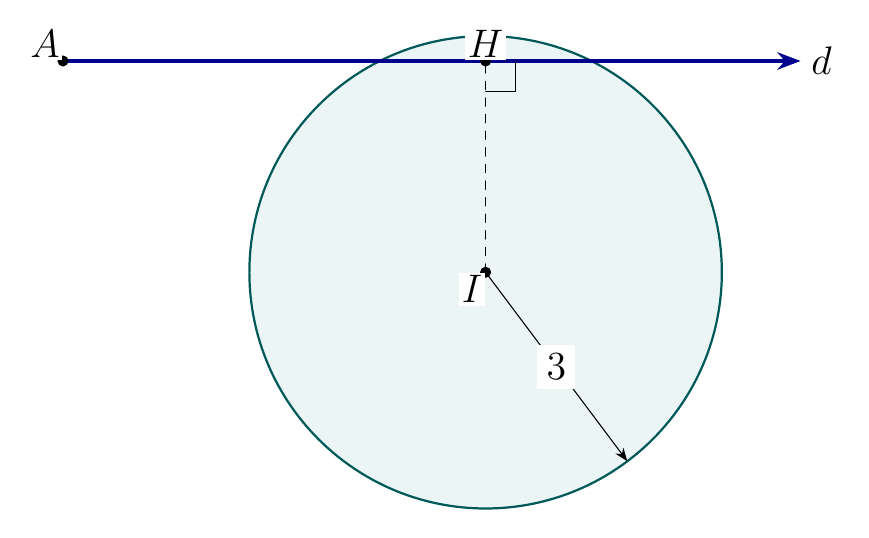
\begin{tikzpicture}[>=Stealth,line cap=round,font=\Large]
\fill[teal!8] (0,0) circle (3);\draw[teal!70!black,thick] (0,0) circle (3);
\draw[->,blue!55!black,very thick] (-5.367,2.683)--(4,2.683) node[right,black] {$d$};
\draw[dashed] (0,0)--(0,2.683);\draw (0,2.3)--(.383,2.3)--(.383,2.683);
\draw[->] (0,0)--(1.8,-2.4) node[midway,fill=white] {$3$};
\fill (0,0) circle (2pt) node[below left,fill=white,inner sep=1pt] {$I$};
\fill (0,2.683) circle (2pt) node[above,fill=white,inner sep=1pt] {$H$};
\fill (-5.367,2.683) circle (2pt) node[above left,fill=white,inner sep=1pt] {$A$};
\end{tikzpicture}}
\end{minipage}
\item Một dây chuyền có $10\%$ linh kiện lỗi. Mỗi lần kiểm tra, máy báo lỗi với xác suất $0{,}8$ nếu linh kiện thực sự lỗi, với xác suất $0{,}2$ nếu linh kiện không lỗi. Chọn ngẫu nhiên một linh kiện và kiểm tra hai lần. Hai kết quả độc lập khi đã biết trạng thái lỗi hay không lỗi của linh kiện.
\begin{enumerate}[label=\alph*)]
\item Xác suất một lần kiểm tra báo lỗi bằng $0{,}3$.
\item Xác suất cả hai lần kiểm tra đều báo lỗi bằng $0{,}1$.
\item Biết ít nhất một lần kiểm tra báo lỗi, xác suất linh kiện thực sự lỗi bằng $\dfrac25$.
\item Biết cả hai lần kiểm tra đều báo lỗi, xác suất linh kiện thực sự lỗi bằng $0{,}64$.
\end{enumerate}
\item \begin{minipage}[t]{0.55\linewidth}
Một xe chuyển động thẳng theo một chiều trong $6$ giây. Đồ thị vận tốc $v$ (m/s) theo thời gian $t$ (giây) là đường gấp khúc nối ba điểm $(0;0)$, $(2;6)$, $(6;0)$ như hình bên.
\begin{enumerate}[label=\alph*)]
\item Vận tốc của xe tại $t=2$ giây bằng $6$ m/s.
\item Trong $4$ giây đầu, xe đi được $18$ m.
\item Tổng quãng đường trong $6$ giây bằng $24$ m.
\item Thời điểm xe đã đi được $\dfrac34$ tổng quãng đường là $t=6-\sqrt6$ giây.
\end{enumerate}
\end{minipage}\hfill
\begin{minipage}[t]{0.42\linewidth}\vspace{-0.4\baselineskip}\centering
\resizebox{\linewidth}{!}{\begin{tikzpicture}[>=Stealth,font=\large]
\draw[->] (-.5,0)--(7.3,0) node[right] {$t$ (s)};
\draw[->] (0,-.5)--(0,7.1) node[above] {$v$ (m/s)};
\draw[blue!55!black,very thick] (0,0)--(2,6)--(6,0);
\draw[dashed] (0,6)--(2,6)--(2,0);
\node[below left] at (0,0) {$O$};\node[left] at (0,6) {$6$};
\node[below] at (2,0) {$2$};\node[below] at (6,0) {$6$};
\end{tikzpicture}}
\end{minipage}
\end{enumerate}

\Needspace{9\baselineskip}
\section*{\large PHẦN III. CÂU TRẮC NGHIỆM TRẢ LỜI NGẮN}
\textit{Thí sinh trả lời từ câu 1 đến câu 6. Mỗi câu trả lời đúng được 0,5 điểm. Chỉ làm tròn ở kết quả cuối cùng.}
\begin{enumerate}
\item Thời gian hoàn thành một tác vụ của $40$ người (đơn vị: phút) được thống kê như sau, trong đó $a,b$ là hai tần số chưa biết:
\begin{center}\begin{tabular}{|c|c|c|c|c|}\hline
Thời gian & $[0;2)$ & $[2;4)$ & $[4;6)$ & $[6;8)$\\\hline
Số người & $4$ & $a$ & $b$ & $6$\\\hline\end{tabular}\end{center}
Biết thời gian trung bình của mẫu số liệu ghép nhóm bằng $4{,}3$ phút. Phương sai của mẫu số liệu ghép nhóm bằng bao nhiêu phút$^2$? \textit{(Làm tròn đến hàng phần trăm.)}

\item Bốn cơ thủ $T,D,E,C$ dự giải đấu với hai trận bán kết: $T$ gặp $D$, $E$ gặp $C$. Hai người thắng gặp nhau ở chung kết. Điểm đánh giá của bốn cơ thủ lần lượt là $m_T=3$, $m_D=5$, $m_E=4$, $m_C=6$. Khi $X$ gặp $Y$, xác suất $X$ thắng là $\dfrac{m_X}{m_X+m_Y}$; không có trận hòa, điểm đánh giá không thay đổi và xác suất thắng một trận khi đã biết đối thủ không phụ thuộc kết quả các trận trước. Biết $T$ vô địch, xác suất đối thủ của $T$ trong trận chung kết là $E$ bằng bao nhiêu? \textit{(Làm tròn đến hàng phần trăm.)}

\Needspace{15\baselineskip}
\item \begin{minipage}[t]{0.55\linewidth}
Một mái che nằm ngang cao $7$ m so với mặt đất, nhô ra $8$ m từ một bức tường thẳng đứng. Xe cứu hỏa đỗ bên ngoài mái che, điểm tựa dưới của thang trên xe cao $1$ m so với mặt đất. Thang được coi là đoạn thẳng từ điểm tựa đến một điểm trên tường phía trên mái che; điểm tựa có thể thay đổi khoảng cách đến tường. Tường đủ cao, bỏ qua độ dày thang và cho phép thang vừa chạm mép mái. Chiều dài thang nhỏ nhất để vượt qua mái che bằng bao nhiêu mét? \textit{(Làm tròn đến hàng phần mười.)}
\end{minipage}\hfill
\begin{minipage}[t]{0.42\linewidth}\vspace{-0.4\baselineskip}\centering
\resizebox{\linewidth}{!}{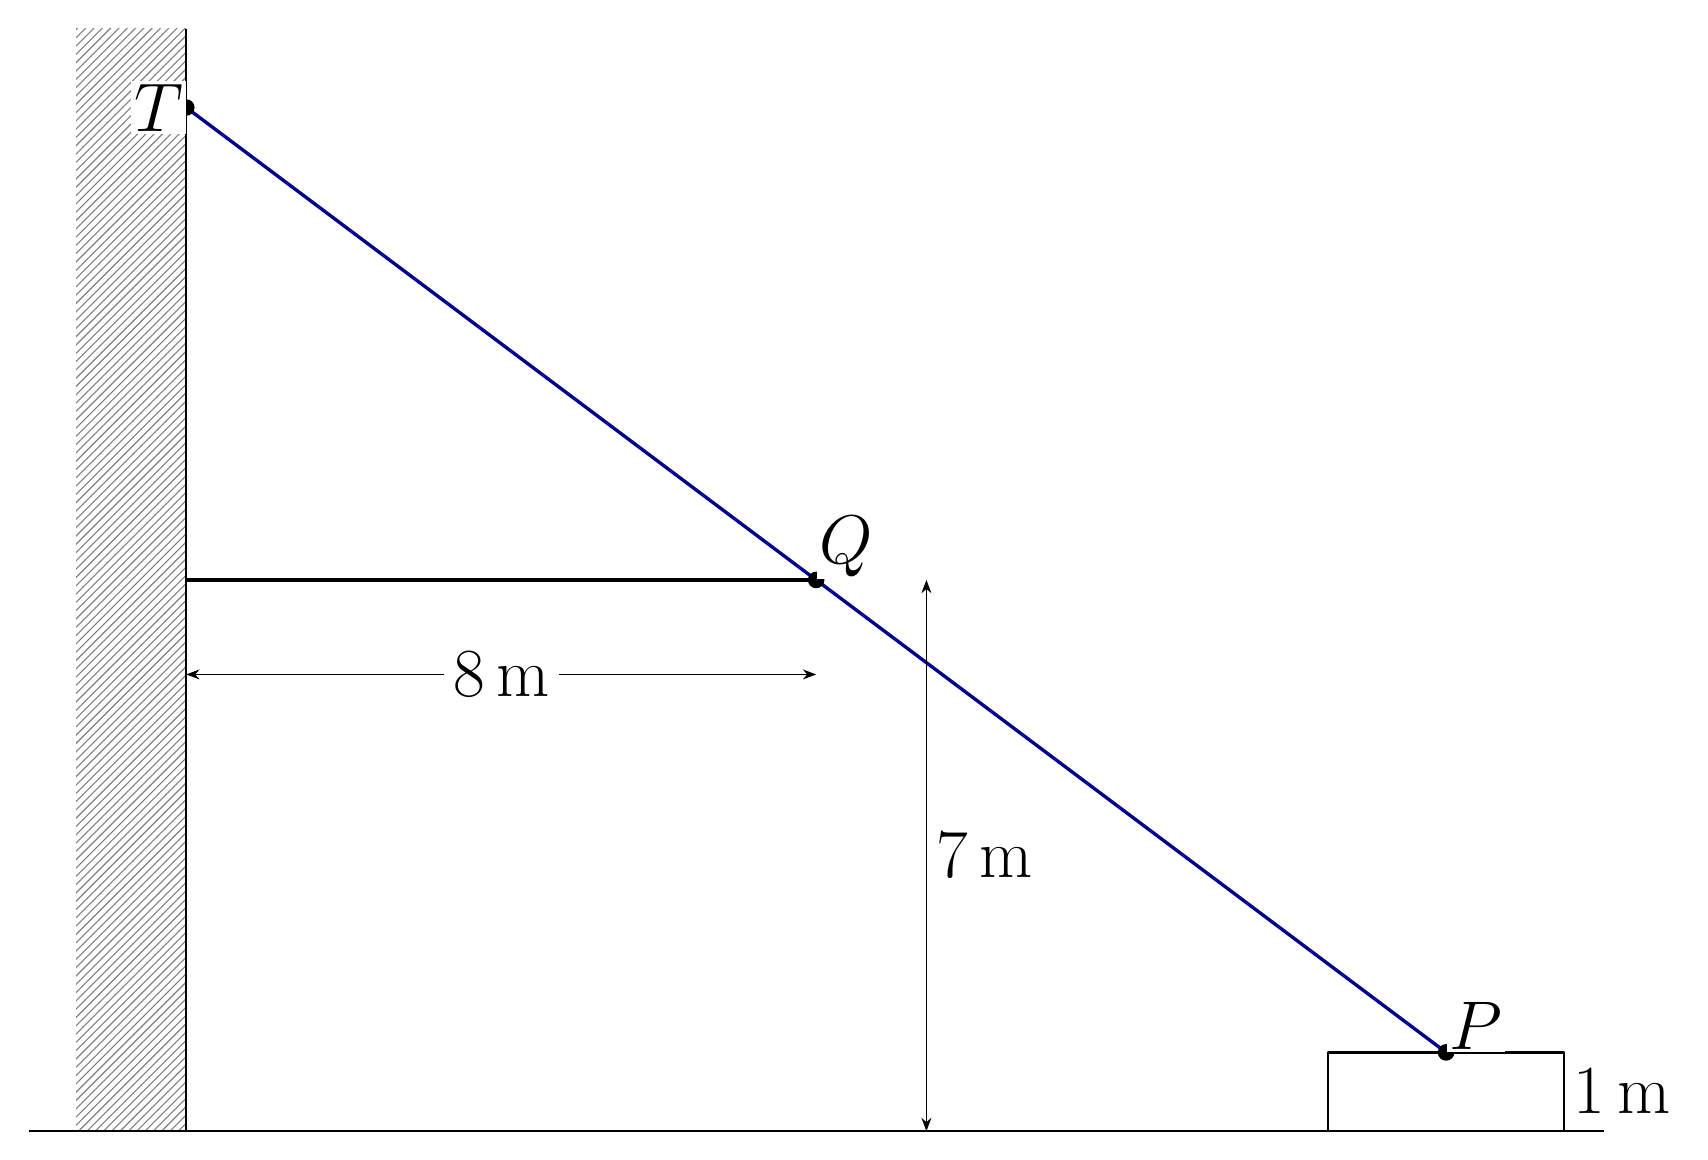
\begin{tikzpicture}[>=Stealth,font=\Huge,line join=round]
\fill[pattern=north east lines,pattern color=gray] (-1.4,0) rectangle (0,14);
\draw[thick] (0,0)--(0,14);\draw[thick] (-2,0)--(18,0);
\draw[very thick] (0,7)--(8,7);\draw[blue!55!black,very thick] (0,13)--(16,1);
\draw[thick] (14.5,0) rectangle (17.5,1);
\fill (0,13) circle (3pt) node[left,fill=white,inner sep=1pt] {$T$};
\fill (8,7) circle (3pt) node[above right,fill=white,inner sep=1pt] {$Q$};
\fill (16,1) circle (3pt) node[above right,fill=white,inner sep=1pt] {$P$};
\draw[<->] (0,5.8)--(8,5.8) node[midway,fill=white] {$8\,\mathrm m$};
\draw[<->] (9.4,0)--(9.4,7) node[midway,right,fill=white] {$7\,\mathrm m$};
\node[right,fill=white] at (17.5,.5) {$1\,\mathrm m$};
\end{tikzpicture}}
\end{minipage}

\Needspace{13\baselineskip}
\item \begin{minipage}[t]{0.55\linewidth}
Một sợi dây không dãn dài $15$ m được kéo theo đường gấp khúc $ABCD$ qua một bức tường cao $4$ m, dày $BC=1$ m. Các điểm $B,C$ cố định ở hai mép trên của tường; $E$ là chân đường thẳng đứng qua $C$, vật cần kéo ở $D$ trên mặt đất bên trái. Điểm $F$ nằm trên mặt tường bên phải, cách $B$ theo phương thẳng đứng $1$ m. Đầu dây $A$ chuyển động trên ray thẳng xuất phát từ $F$, nghiêng xuống sang phải và hợp với phương ngang góc $30^\circ$. Khi $AF=4$ m, vật $D$ tiến về $E$ với tốc độ $1$ m/s. Khi đó đầu dây $A$ rời xa $F$ với tốc độ bao nhiêu m/s? \textit{(Làm tròn đến hàng phần trăm.)}
\end{minipage}\hfill
\begin{minipage}[t]{0.42\linewidth}\vspace{-0.4\baselineskip}\centering
\resizebox{\linewidth}{!}{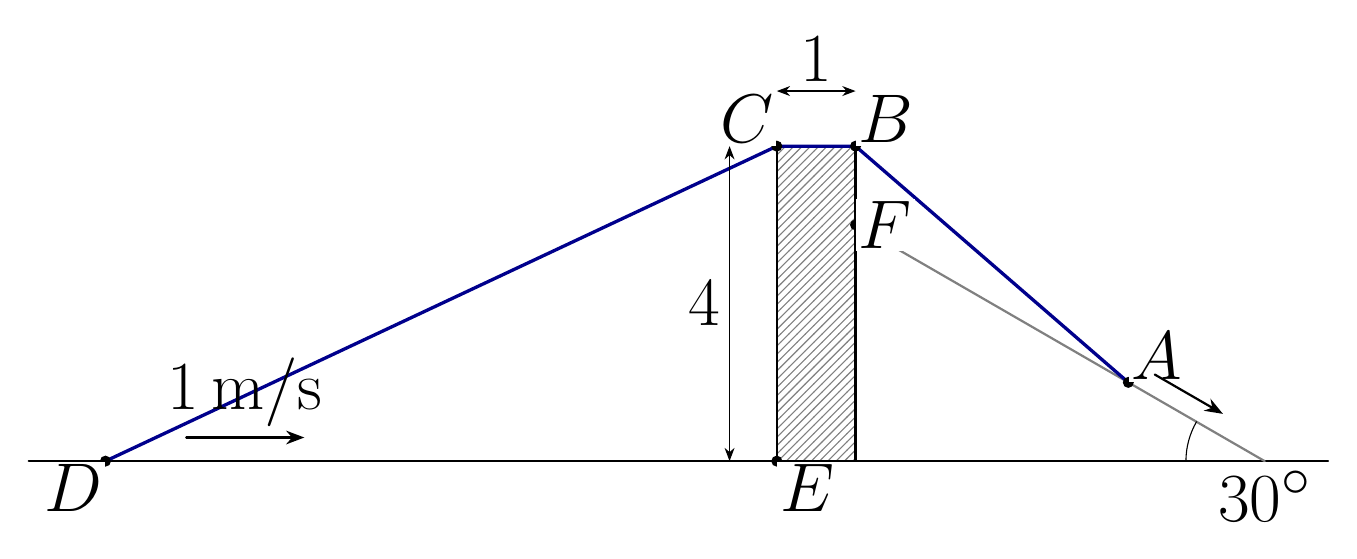
\begin{tikzpicture}[>=Stealth,font=\Huge,line cap=round,line join=round]
\fill[pattern=north east lines,pattern color=gray] (0,0) rectangle (1,4);
\draw[thick] (0,0) rectangle (1,4);\draw[thick] (-9.5,0)--(7,0);
\draw[gray,thick] (1,3)--(6.196,0);
\draw[blue!55!black,very thick] (-8.526,0)--(0,4)--(1,4)--(4.464,1);
\foreach \p/\label/\pos in {(0,4)/C/above left,(1,4)/B/above right,(0,0)/E/below right,(-8.526,0)/D/below left,(1,3)/F/right,(4.464,1)/A/above right}{
\fill \p circle (2pt) node[\pos,fill=white,inner sep=1pt] {$\label$};}
\draw[<->] (0,4.7)--(1,4.7) node[midway,above] {$1$};
\draw[<->] (-.6,0)--(-.6,4) node[midway,left,fill=white] {$4$};
\draw[->,thick] (-7.5,.3)--(-6,.3) node[midway,above] {$1\,\mathrm{m/s}$};
\draw[->,thick] (4.8,1.1)--(5.666,.6);
\draw (5.196,0) arc[start angle=180,end angle=150,radius=1];
\node[below] at (6.196,0) {$30^\circ$};
\end{tikzpicture}}
\end{minipage}

\item Hai tàu đánh cá chuyển động trên hai nhánh khác nhau của đường cong $(C):y=\dfrac{x^2+x+1}{x+1}$ trong hệ trục $Oxy$, đơn vị mỗi trục là km. Một tàu luôn có hoành độ nhỏ hơn $-1$, tàu còn lại luôn có hoành độ lớn hơn $-1$. Khoảng cách nhỏ nhất có thể giữa hai tàu bằng bao nhiêu km? \textit{(Làm tròn đến hàng phần trăm.)}

\Needspace{15\baselineskip}
\item \begin{minipage}[t]{0.55\linewidth}
Một khối hộp chữ nhật $ABCD.A'B'C'D'$ có $AB=6$ m, $BC=4$ m, $AA'=2$ m. Điểm $M$ thuộc $AB$, $AM=2$ m. Một robot nhỏ đi từ $M$ đến $D'$ theo đường gấp khúc $MNP D'$: $N$ thuộc cạnh $BC$, $P$ thuộc cạnh $CC'$. Các đoạn $MN,NP,PD'$ lần lượt nằm trên ba mặt $ABCD$, $BCC'B'$, $CDD'C'$. Cho phép $N,P$ trùng với đầu mút của các cạnh tương ứng; một đoạn có thể có độ dài bằng $0$. Tổng quãng đường ngắn nhất bằng bao nhiêu mét? \textit{(Làm tròn đến hàng phần mười.)}
\end{minipage}\hfill
\begin{minipage}[t]{0.42\linewidth}\vspace{-0.4\baselineskip}\centering
\resizebox{\linewidth}{!}{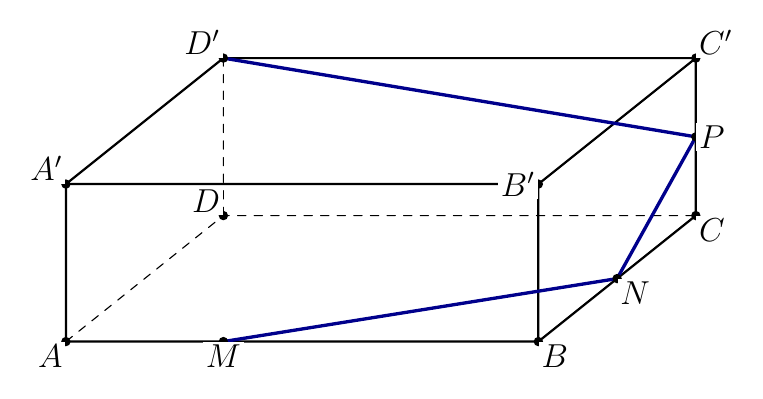
\begin{tikzpicture}[>=Stealth,font=\large,line cap=round,line join=round,
x={(1cm,0cm)},y={(.5cm,.4cm)},z={(0cm,1cm)}]
\coordinate (A) at (0,0,0);\coordinate (B) at (6,0,0);\coordinate (C) at (6,4,0);\coordinate (D) at (0,4,0);
\coordinate (Ap) at (0,0,2);\coordinate (Bp) at (6,0,2);\coordinate (Cp) at (6,4,2);\coordinate (Dp) at (0,4,2);
\coordinate (M) at (2,0,0);\coordinate (N) at (6,2,0);\coordinate (P) at (6,4,1);
\draw[thick] (A)--(B)--(C)--(Cp)--(Dp)--(Ap)--cycle;
\draw[thick] (Ap)--(Bp)--(Cp) (B)--(Bp);
\draw[dashed] (A)--(D)--(C) (D)--(Dp);
\draw[blue!55!black,very thick] (M)--(N)--(P)--(Dp);
\foreach \p/\label/\pos in {A/A/below left,B/B/below right,C/C/below right,D/D/above left,Ap/A'/above left,Bp/B'/left,Cp/C'/above right,Dp/D'/above left,M/M/below,N/N/below right,P/P/right}{
\fill (\p) circle (1.7pt) node[\pos,fill=white,inner sep=1pt] {$\label$};}
\end{tikzpicture}}
\end{minipage}
\end{enumerate}
\begin{center}\textbf{--- HẾT ---}\end{center}

% BAT DAU DAP AN
\newpage
\begin{center}{\Large\textbf{BẢNG ĐÁP ÁN TỔNG HỢP}}\\[4pt]\textbf{ĐỀ SỐ 15}\end{center}
\textbf{PHẦN I. TRẮC NGHIỆM NHIỀU PHƯƠNG ÁN}
\begin{center}\renewcommand{\arraystretch}{1.5}\begin{tabular}{|*{12}{c|}}\hline
1 & 2 & 3 & 4 & 5 & 6 & 7 & 8 & 9 & 10 & 11 & 12\\\hline
C & A & D & B & A & C & B & D & C & B & D & A\\\hline
\end{tabular}\end{center}
\textbf{PHẦN II. TRẮC NGHIỆM ĐÚNG SAI}
\begin{center}\renewcommand{\arraystretch}{1.5}\begin{tabular}{|c|c|c|c|c|}\hline
Câu & a) & b) & c) & d)\\\hline
1 & Đ & Đ & S & Đ\\\hline
2 & S & Đ & Đ & S\\\hline
3 & S & Đ & S & Đ\\\hline
4 & Đ & S & S & Đ\\\hline
\end{tabular}\end{center}
\textbf{PHẦN III. TRẮC NGHIỆM TRẢ LỜI NGẮN}
\begin{center}\renewcommand{\arraystretch}{1.5}\begin{tabular}{|c|c|c|c|c|c|}\hline
1 & 2 & 3 & 4 & 5 & 6\\\hline
2,91 & 0,46 & 19,7 & 0,92 & 4,39 & 12,0\\\hline
\end{tabular}\end{center}

\newpage
\begin{center}{\Large\textbf{HƯỚNG DẪN GIẢI CHI TIẾT}}\\[4pt]\textbf{ĐỀ SỐ 15}\end{center}
\section*{\large PHẦN I. TRẮC NGHIỆM NHIỀU PHƯƠNG ÁN}
\loigiai{Câu 1. Chọn C.}
Điều kiện $x>-1/2$. Vì cơ số $3>1$, bất phương trình tương đương $2x+1>9$, tức $x>4$, đã thỏa điều kiện. Tập nghiệm là $(4;+\infty)$.
\loigiai{Câu 2. Chọn A.}
Ta có $y'=3x^2-6x=3x(x-2)<0$ khi $0<x<2$. Hàm số nghịch biến trên $(0;2)$.
\loigiai{Câu 3. Chọn D.}
\[\int_0^\pi\sin x\,\mathrm dx=[-\cos x]_0^\pi=1-(-1)=2.\]
\loigiai{Câu 4. Chọn B.}
Từ phương trình mặt phẳng, một vectơ pháp tuyến là bộ hệ số của $x,y,z$: $\vec n=(2;-3;1)$.
\loigiai{Câu 5. Chọn A.}
Các giá trị đại diện là $3,5,7$, nên $\overline x=(5\cdot3+10\cdot5+5\cdot7)/20=5$ kg.
\loigiai{Câu 6. Chọn C.}
Gọi $E$ là biến cố cả hai thiết bị tốt, $F$ là biến cố ít nhất một thiết bị tốt. Do độc lập, $P(E)=0{,}7\cdot0{,}4=0{,}28$ và $P(F)=1-0{,}3\cdot0{,}6=0{,}82$. Vì $E\subset F$, $P(E\mid F)=0{,}28/0{,}82=14/41$.
\loigiai{Câu 7. Chọn B.}
Có $\binom93$ cách chọn ba người, trong đó $\binom42\binom51$ cách chọn đúng hai nữ. Xác suất là $30/84=5/14$.
\loigiai{Câu 8. Chọn D.}
$u_4=u_1q^3=81(1/3)^3=3$.
\loigiai{Câu 9. Chọn C.}
$R=IA=\sqrt{3^2+4^2}=5$. Phương trình là $(x-1)^2+(y-2)^2+(z+1)^2=25$.
\loigiai{Câu 10. Chọn B.}
Viết $f(x)=x+1+3/(x-1)$, suy ra $f'(x)=1-3/(x-1)^2$. Điều kiện song song là $f'(x)=-2$, cho $x=0$ hoặc $x=2$. Hai tiếp tuyến lần lượt là $y=-2x-2$ và $y=-2x+10$. Khoảng cách giữa chúng bằng
\[\frac{|10-(-2)|}{\sqrt{(-2)^2+1^2}}=\frac{12}{\sqrt5}.\]
\loigiai{Câu 11. Chọn D.}
Mặt cầu có tâm $O$, bán kính $2$; $d(O,(P))=9/3=3$. Vì $(P)$ không cắt mặt cầu, khoảng cách lớn nhất bằng $3+2=5$. Dấu bằng đạt tại $M(-2/3;-4/3;-4/3)$, điểm xa mặt phẳng theo phương pháp tuyến.
\loigiai{Câu 12. Chọn A.}
Lợi nhuận là $P(x)=x(30-0{,}1x)-(5x+200)=-0{,}1x^2+25x-200$. Đỉnh parabol có hoành độ $125$ nằm ngoài miền cho phép. Trên $[1;100]$, $P'(x)=25-0{,}2x\geq5>0$, nên lợi nhuận lớn nhất tại $x=100$.

\Needspace{10\baselineskip}
\section*{\large PHẦN II. TRẮC NGHIỆM ĐÚNG SAI}
\loigiai{Câu 1. a) Đúng; b) Đúng; c) Sai; d) Đúng.}
Chi phí bình quân trên một sản phẩm phải nhân với $x$ để có tổng chi phí:
\[C(x)=xg(x)=0{,}01x^3-0{,}2x^2+20x+100.\]
Doanh thu là $R(x)=xp(x)=60x-0{,}1x^2$. Vì vậy
\[P(x)=R(x)-C(x)=-0{,}01x^3+0{,}1x^2+40x-100.\]
Xét hàm trên đoạn thực $[1;80]$:
\[P'(x)=-0{,}03x^2+0{,}2x+40=-0{,}03(x-40)(x+100/3).\]
Đạo hàm dương khi $1\leq x<40$ và âm khi $40<x\leq80$. Giá trị lớn nhất đạt tại $x=40$, là số nguyên hợp lệ, không phải $50$. Ta có $P(40)=1020$ nghìn đồng, tức $1{,}02$ triệu đồng.

\loigiai{Câu 2. a) Sai; b) Đúng; c) Đúng; d) Sai.}
Mặt cầu giới hạn vùng phát hiện có vế phải $R^2=9$, không phải $3$. Ta tính
\[IM^2=(-6+2t)^2+t^2=5t^2-24t+36=5(t-12/5)^2+36/5.\]
Tại $t=0$, khoảng cách $IA=6>3$, drone ở ngoài vùng phát hiện. Khoảng cách nhỏ nhất đạt tại $t=12/5\geq0$. Radar phát hiện drone khi
\[5t^2-24t+36\leq9\ \Longleftrightarrow\ 5t^2-24t+27\leq0\ \Longleftrightarrow\ 9/5\leq t\leq3.\]
Thời gian phát hiện dài $3-9/5=6/5=1{,}2$ phút, không phải $2$ phút.

\loigiai{Câu 3. a) Sai; b) Đúng; c) Sai; d) Đúng.}
Gọi $D$ là biến cố linh kiện thực sự lỗi, $E$ là biến cố cả hai lần báo lỗi, $F$ là biến cố ít nhất một lần báo lỗi. Theo xác suất toàn phần và độc lập có điều kiện:
\begin{enumerate}[label=\alph*),leftmargin=*]
\item $P(\text{một lần báo lỗi})=0{,}1\cdot0{,}8+0{,}9\cdot0{,}2=0{,}26$, không phải $0{,}3$.
\item $P(E)=0{,}1\cdot0{,}8^2+0{,}9\cdot0{,}2^2=0{,}064+0{,}036=0{,}1$.
\item $P(F\mid D)=1-0{,}2^2=0{,}96$, $P(F\mid\overline D)=1-0{,}8^2=0{,}36$. Do đó $P(F)=0{,}1\cdot0{,}96+0{,}9\cdot0{,}36=0{,}42$, và
\[P(D\mid F)=\frac{0{,}1\cdot0{,}96}{0{,}42}=\frac8{35},\]
không phải $2/5$.
\item $P(D\mid E)=0{,}064/0{,}1=0{,}64$.
\end{enumerate}

\loigiai{Câu 4. a) Đúng; b) Sai; c) Sai; d) Đúng.}
Từ hai đoạn thẳng của đồ thị,
\[v(t)=\begin{cases}3t,&0\leq t\leq2,\\9-1{,}5t,&2\leq t\leq6.\end{cases}\]
Vận tốc luôn không âm nên quãng đường bằng diện tích dưới đồ thị. Ta có $v(2)=6$ m/s. Trong $4$ giây đầu,
\[S(4)=\tfrac12\cdot2\cdot6+\tfrac{6+3}{2}\cdot2=6+9=15\ \mathrm m.\]
Tổng quãng đường $S(6)=\tfrac12\cdot6\cdot6=18$ m. Ba phần tư tổng quãng đường là $13{,}5$ m, lớn hơn $S(2)=6$, nên thời điểm cần tìm thuộc $(2;6)$. Đặt $u=t-2\in[0;4]$, ta có
\[6+6u-0{,}75u^2=13{,}5\ \Longleftrightarrow\ u^2-8u+10=0.\]
Nghiệm hợp lệ là $u=4-\sqrt6$, suy ra $t=6-\sqrt6$ giây.

\Needspace{10\baselineskip}
\section*{\large PHẦN III. TRẮC NGHIỆM TRẢ LỜI NGẮN}
\loigiai{Câu 1. Đáp số: 2,91.}
Các giá trị đại diện là $1,3,5,7$. Từ cỡ mẫu và trung bình, ta có
\[a+b=30,\qquad\frac{4+3a+5b+42}{40}=4{,}3.\]
Giải hệ $a+b=30$, $3a+5b=126$ được $a=12$, $b=18$. Phương sai là
\[s^2=\frac{4\cdot1^2+12\cdot3^2+18\cdot5^2+6\cdot7^2}{40}-4{,}3^2
=\frac{856}{40}-18{,}49=2{,}91.\]

\loigiai{Câu 2. Đáp số: 0,46.}
Gọi $V$ là biến cố $T$ vô địch, $H$ là biến cố $E$ thắng bán kết. Nếu $T$ vô địch thì $T$ đã thắng bán kết, nên đối thủ chung kết là $E$ đúng khi $H$ xảy ra.
Xác suất $T$ thắng bán kết là $3/8$, $E$ thắng bán kết là $4/10=2/5$. Theo hai nhánh đối thủ ở chung kết,
\[P(V\cap H)=\frac38\cdot\frac25\cdot\frac37=\frac9{140},\qquad
P(V\cap\overline H)=\frac38\cdot\frac35\cdot\frac39=\frac3{40}.\]
Vì vậy
\[P(H\mid V)=\frac{9/140}{9/140+3/40}=\frac6{13}\approx0{,}461538.\]
Làm tròn: $0{,}46$. Xác suất $E$ thắng bán kết $2/5$ không phải đáp án, vì đã biết $T$ vô địch.

\loigiai{Câu 3. Đáp số: 19,7.}
Gọi $d>0$ là khoảng cách theo phương ngang từ điểm tựa dưới $P$ đến mép ngoài mái che. Với cùng một vị trí $P$, thang ngắn nhất có thể vượt mái sẽ đi qua đúng mép ngoài $Q$; nếu thang vượt cao hơn, có thể hạ đầu trên xuống cho đến khi vừa chạm $Q$, độ dài giảm.
Độ cao của $Q$ so với $P$ là $7-1=6$ m. Các tam giác đồng dạng cho độ tăng chiều cao từ $P$ đến tường bằng $6(d+8)/d$, còn khoảng cách ngang từ $P$ đến tường là $d+8$. Do đó
\[L(d)=(d+8)\sqrt{1+\frac{36}{d^2}},\qquad d>0.\]
Để tránh căn thức, xét $F(d)=L(d)^2$; tối ưu $F$ cũng tối ưu $L$. Ta có
\[F'(d)=\frac{2(d+8)(d^3-288)}{d^3}.\]
Đạo hàm âm khi $0<d<\sqrt[3]{288}$, dương khi $d>\sqrt[3]{288}$. Do đó
\[d_* =\sqrt[3]{288}\approx6{,}603854,\qquad
L_{\min}=\left(8^{2/3}+6^{2/3}\right)^{3/2}\approx19{,}731325.\]
Làm tròn: $19{,}7$ m. Phải dùng độ chênh cao $6$ m, không dùng chiều cao mái $7$ m tính từ mặt đất.

\loigiai{Câu 4. Đáp số: 0,92.}
Đặt $x=DE>0$, $y=AF>0$, tính theo mét. Do ray nghiêng xuống $30^\circ$ so với phương ngang, còn $FB$ thẳng đứng hướng lên, ta có $\widehat{AFB}=120^\circ$. Theo định lí cosin,
\[AB^2=y^2+1^2-2y\cos120^\circ=y^2+y+1.\]
Mặt khác $CD=\sqrt{x^2+4^2}$. Chiều dài dây không đổi cho
\[\sqrt{y^2+y+1}+1+\sqrt{x^2+16}=15
\ \Longleftrightarrow\ \sqrt{y^2+y+1}+\sqrt{x^2+16}=14.\]
Tại $y=4$, ta có $AB=\sqrt{21}$, $CD=14-\sqrt{21}$ và
\[x=\sqrt{(14-\sqrt{21})^2-16}.\]
Lấy đạo hàm hai vế theo thời gian $t$:
\[\frac{2y+1}{2\sqrt{y^2+y+1}}\frac{\mathrm dy}{\mathrm dt}
+\frac{x}{\sqrt{x^2+16}}\frac{\mathrm dx}{\mathrm dt}=0.\]
Vật tiến về $E$ nên $\mathrm dx/\mathrm dt=-1$ m/s. Vì vậy
\[\left.\frac{\mathrm dy}{\mathrm dt}\right|_{y=4}
=\frac{2\sqrt{21}}9\,
\frac{\sqrt{(14-\sqrt{21})^2-16}}{14-\sqrt{21}}
\approx0{,}9219259.\]
Tốc độ rời xa $F$ là $0{,}92$ m/s. Không làm tròn giá trị $x$ trung gian; cần giữ đúng dấu âm của tốc độ $DE$.

\loigiai{Câu 5. Đáp số: 4,39.}
Viết lại hàm số
\[f(x)=x+\frac1{x+1}.\]
Tịnh tiến hệ tọa độ về tâm $I(-1;-1)$ bằng $u=x+1$, $v=y+1$; đường cong trở thành $v=u+1/u$. Phép tịnh tiến giữ nguyên khoảng cách.
Điểm trên nhánh phải có dạng $A(a;a+1/a)$, điểm trên nhánh trái có dạng $B(-b;-b-1/b)$ với $a,b>0$. Do đó
\[AB^2=(a+b)^2+\left(a+b+\frac1a+\frac1b\right)^2.\]
Đặt $S=a+b>0$. Vì $ab\leq S^2/4$,
\[\frac1a+\frac1b=\frac S{ab}\geq\frac4S.\]
Các biểu thức đều dương, suy ra
\[AB^2\geq S^2+\left(S+\frac4S\right)^2
=2S^2+8+\frac{16}{S^2}\geq8+8\sqrt2.\]
Bất đẳng thức cuối dùng $2S^2+16/S^2\geq2\sqrt{32}=8\sqrt2$. Để cả hai dấu bằng đồng thời xảy ra cần $a=b$ và $S^4=8$, tức $a=b=2^{-1/4}$; đây là hai điểm hợp lệ trên hai nhánh.
Vì vậy
\[d_{\min}=\sqrt{8+8\sqrt2}=2\sqrt{2+2\sqrt2}\approx4{,}394736.\]
Làm tròn: $4{,}39$ km. Không được mặc định hai tàu có cùng độ lệch hoành độ khỏi tâm; tính đối xứng tối ưu phải được chứng minh bằng điều kiện dấu bằng.

\loigiai{Câu 6. Đáp số: 12,0.}
Chọn hệ tọa độ cho hình hộp: $A(0;0;0)$, $B(6;0;0)$, $C(6;4;0)$, $D(0;4;0)$, $D'(0;4;2)$. Khi đó $M(2;0;0)$.
Viết $N(6;n;0)$, $P(6;4;p)$ với $0\leq n\leq4$, $0\leq p\leq2$. Tổng độ dài đường đi là
\[L=\sqrt{16+n^2}+\sqrt{(4-n)^2+p^2}+\sqrt{36+(2-p)^2}.\]
\textbf{Kiểm tra tính hợp lệ khi trải phẳng.} Trên hình trải ba mặt, có thể đặt $M=(0;-4)$, $D'=(10;2)$; cạnh $BC$ nằm trên $y=0$ với hoành độ trong $[0;4]$, cạnh $CC'$ nằm trên $x=4$ với tung độ trong $[0;2]$. Đoạn thẳng nối hai điểm đầu cuối cắt $y=0$ tại hoành độ $20/3>4$, nằm ngoài cạnh $BC$. Vì vậy $\sqrt{10^2+6^2}=\sqrt{136}$ không phải độ dài của một đường đi được phép.

\textbf{Tìm cận dưới đạt được.} Bất đẳng thức Cauchy cho
\[\sqrt{16+n^2}\geq\frac{4+n}{\sqrt2},\qquad
\sqrt{36+(2-p)^2}\geq\frac{18+(2-p)}{\sqrt{10}}=\frac{20-p}{\sqrt{10}}.\]
Đặt $q=4-n\geq0$. Vì $1/2+1/10=3/5<1$, Cauchy cũng cho
\[\frac q{\sqrt2}+\frac p{\sqrt{10}}
\leq\sqrt{q^2+p^2}\sqrt{\frac35}\leq\sqrt{q^2+p^2}.\]
Cộng ba cận dưới:
\[L\geq\frac{4+n+4-n}{\sqrt2}+\frac{p+20-p}{\sqrt{10}}
=4\sqrt2+2\sqrt{10}.\]
Cận dưới đạt được tại $n=4$, $p=0$, nghĩa là $N=P=C$. Điểm này được đề bài cho phép; robot đi theo $M\to C\to D'$ và đoạn $NP$ có độ dài $0$. Khi đó
\[L_{\min}=MC+CD'=\sqrt{4^2+4^2}+\sqrt{6^2+2^2}
=4\sqrt2+2\sqrt{10}\approx11{,}9814096.\]
Làm tròn đến hàng phần mười: $12{,}0$ m. Việc xét đầu mút là bắt buộc; chỉ tìm nghiệm cực trị trong lòng hai cạnh sẽ bỏ lỡ đường đi ngắn nhất.
\begin{center}\textbf{--- HẾT LỜI GIẢI ---}\end{center}
\end{document}
